\documentclass[10pt,a4paper]{article}
\usepackage[latin1]{inputenc}
\usepackage{amsmath}
\usepackage{amsfonts}
\usepackage{amssymb}
\usepackage{graphicx}
\usepackage{amssymb}
\author{Paul Wieland}
\title{INF3490 Mandatory Assignment 2:
	Multilayer Perceptron}
\date{Deadline: Tuesday, October 16th, 2018 23:59:00}
\begin{document}
	\maketitle
	\tableofcontents
	\newpage
	%%%%%%%%%%%%%%%%%%%%%%%%%%%%%%%%%%%%%%%%%%%%%%%% 	%INTRODUCTION
	\section{Introduction}
	\subsection{Task}									%task
	We will build a Multilayer Perceptron to steer a robotic prosthetic hand. There are 40 inputs of electromyographic signals that we will classify. \\
	There are 8 classification values corresponding to a different hand motion: \\
	\begin{center}
		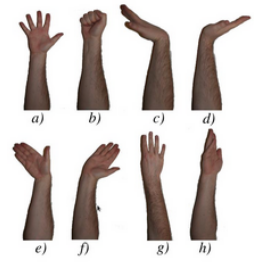
\includegraphics[width=0.4\linewidth]{pictures/hand}
		\\
		Figure 1: Possible motions \footnote{http://folk.uio.no/kyrrehg/pf/papers/glette-ahs08.pdf}
		\\
	\end{center}
	\begin{center}
		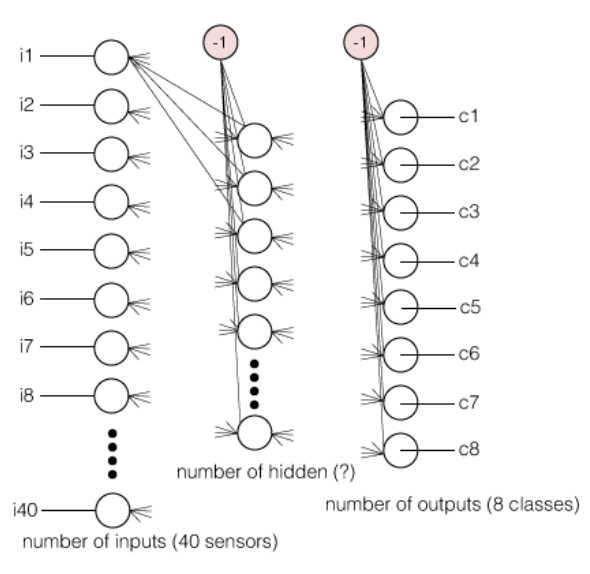
\includegraphics[width=0.7\linewidth]{pictures/mlp}
		\\
		Figure 2: Multilayer Perceptron for our problem \footnote{https://www.uio.no/studier/emner/matnat/ifi/INF3490/h18/assignments/assignment-2/assignment\_2.pdf}
		\\
	\end{center}
	We build a Multilayer Perceptron with 40 entry nodes, that means one node for each input. Then there is one hidden layer with a various number of hidden nodes. For classifying the input, there are 8 output nodes corresponding to the 8 hand motions. We only use one hidden layer to solve this problem.

	\subsection{Training Data}							%training data
	For each input vector:
	\begin{center}

		\begin{equation}
		input = [i_1,i_2,i_3,i_4,...,i_{40}], i_n \in  \mathbb{R},n \in [40]
		\end{equation}
	\end{center}
	we have a target output vector:
	\begin{center}
		\begin{equation}
		 output = [c_1,c_2,c_3,c_4,...,c_8], c_n \in \{0,1\}, n \in [8],\sum_{n=1}^{8} c_n  = 1 
		 \end{equation}  
	\end{center}
	That means, forwarding the input should result in the given target vector. 
	%%%%%%%%%%%%%%%%%%%%%%%%%%%%%%%%%%%%%%%%%%%%%%%%		%IMPLEMENTATION
	\section{Implementation}
	The file \textit{mlp.py} contains the class mlp. There are 5 functions that i will explain in detail.
	\subsection{Initialization}
	The function \textit{ \_\_init\_\_(self, inputs, targets, nhidden)} has three important parameter that we need to initialize the Multilayer Perceptron. \\
	As the input data is given as a vector, it is a good choice to create two 2D-Array for the two weight layers. As the parameters \textit{inputs} and \textit{targets} have the type \textit{$<$class 'numpy.ndarray'$>$}, it is a good idea to work only with numpy arrays. \\
	\subsubsection{Dimension of the weight matrix}			%initalization
		\begin{itemize}
		\item weight\_matrix\_1: \\
		The input vector in (1) has of course a size of 40 ($len(inputs[n]), n \in [len(inputs) -1] \cup \{0\}$). But we need to add the \textit{bias\_value -1} that can be seen in Figure 2. That means: \\ 
		\begin{center}
			\begin{equation}
			 \textit{weight\_matrix\_1} \in \mathbb{R}^{41 \times nhidden} 
			\end{equation} 
		\end{center}
		\item weight\_matrix\_2: \\
		There are \textit{nhidden} hidden nodes and 8 ($len(targets[n]), n \in [len(targets) -1] \cup \{0\}$) exit nodes. So we also need to take into account the \textit{bias\_value -1}. That means: \\
		\begin{center}
			\begin{equation}
			\textit{weight\_matrix\_2} \in \mathbb{R}^{(nhidden+1) \times 8} 
			\end{equation}  
		\end{center}
	\end{itemize} 
	Both, \textit{weigh\_matrix\_1} and \textit{weigh\_matrix\_2}, will be initialized randomly with values in [-1,1].
	
	\subsection{Forward}								%forward
	The forward function takes one input vector and runs it on the network. At first, the input vector must be expanded. The reason for this is that we have to take into account the bias value:	
	\begin{center}
		\begin{equation}
		\textit{input} \in \mathbb{R}^{1\times 41} 
		\end{equation} 
	\end{center}
	Subsequently it is possible to compute the \textit{hidden\_values}:
	\begin{center}
		\begin{equation}
		\textit{hidden\_values} = [h_1,h_2,h_3,h_4,...,h_8]
		\end{equation} 
	\end{center}

	\begin{center}
		\begin{equation}
		h_i = \sum_{n=1}^{41} input[n] \times weight\_matrix\_1[n][i] 
		\end{equation} 
	\end{center}
	This operation is done by the function \textit{ vec\_matr\_mult()} (that function can be found in the file \textit{operations.py}) that is doing a vector matrix multiplication with two for-loops. \\
	After that is the activation function applied to all hidden nodes:
	\begin{center}
		\begin{equation}
		h_{new, i} = \frac{1}{1 + \ exp(-\beta h_i)}
		\end{equation} 
	\end{center}
	The resulting \textit{activation\_hidden\_values} is also expanded by the bias -1: 
	\begin{center}
		\begin{equation}
		\textit{activation\_hidden\_values} \in \mathbb{R}^{1\times (nhidden +1)} 
		\end{equation} 
	\end{center}
	 So the \textit{output} vector can be calculated easily by another vector matrix multiplication:
	  \begin{center}
	  	\begin{equation}
	  	\textit{output} = activation\_hidden\_values \cdot weight\_matrix\_2} 
	  	\end{equation} 
	  \end{center}
	
	
\end{document}